\documentclass[1p]{elsarticle_modified}
%\bibliographystyle{elsarticle-num}

%\usepackage[colorlinks]{hyperref}
%\usepackage{abbrmath_seonhwa} %\Abb, \Ascr, \Acal ,\Abf, \Afrak
\usepackage{amsfonts}
\usepackage{amssymb}
\usepackage{amsmath}
\usepackage{amsthm}
\usepackage{scalefnt}
\usepackage{amsbsy}
\usepackage{kotex}
\usepackage{caption}
\usepackage{subfig}
\usepackage{color}
\usepackage{graphicx}
\usepackage{xcolor} %% white, black, red, green, blue, cyan, magenta, yellow
\usepackage{float}
\usepackage{setspace}
\usepackage{hyperref}

\usepackage{tikz}
\usetikzlibrary{arrows}

\usepackage{multirow}
\usepackage{array} % fixed length table
\usepackage{hhline}

%%%%%%%%%%%%%%%%%%%%%
\makeatletter
\renewcommand*\env@matrix[1][\arraystretch]{%
	\edef\arraystretch{#1}%
	\hskip -\arraycolsep
	\let\@ifnextchar\new@ifnextchar
	\array{*\c@MaxMatrixCols c}}
\makeatother %https://tex.stackexchange.com/questions/14071/how-can-i-increase-the-line-spacing-in-a-matrix
%%%%%%%%%%%%%%%

\usepackage[normalem]{ulem}

\newcommand{\msout}[1]{\ifmmode\text{\sout{\ensuremath{#1}}}\else\sout{#1}\fi}
%SOURCE: \msout is \stkout macro in https://tex.stackexchange.com/questions/20609/strikeout-in-math-mode

\newcommand{\cancel}[1]{
	\ifmmode
	{\color{red}\msout{#1}}
	\else
	{\color{red}\sout{#1}}
	\fi
}

\newcommand{\add}[1]{
	{\color{blue}\uwave{#1}}
}

\newcommand{\replace}[2]{
	\ifmmode
	{\color{red}\msout{#1}}{\color{blue}\uwave{#2}}
	\else
	{\color{red}\sout{#1}}{\color{blue}\uwave{#2}}
	\fi
}

\newcommand{\Sol}{\mathcal{S}} %segment
\newcommand{\D}{D} %diagram
\newcommand{\A}{\mathcal{A}} %arc


%%%%%%%%%%%%%%%%%%%%%%%%%%%%%5 test

\def\sl{\operatorname{\textup{SL}}(2,\Cbb)}
\def\psl{\operatorname{\textup{PSL}}(2,\Cbb)}
\def\quan{\mkern 1mu \triangleright \mkern 1mu}

\theoremstyle{definition}
\newtheorem{thm}{Theorem}[section]
\newtheorem{prop}[thm]{Proposition}
\newtheorem{lem}[thm]{Lemma}
\newtheorem{ques}[thm]{Question}
\newtheorem{cor}[thm]{Corollary}
\newtheorem{defn}[thm]{Definition}
\newtheorem{exam}[thm]{Example}
\newtheorem{rmk}[thm]{Remark}
\newtheorem{alg}[thm]{Algorithm}

\newcommand{\I}{\sqrt{-1}}
\begin{document}

%\begin{frontmatter}
%
%\title{Boundary parabolic representations of knots up to 8 crossings}
%
%%% Group authors per affiliation:
%\author{Yunhi Cho} 
%\address{Department of Mathematics, University of Seoul, Seoul, Korea}
%\ead{yhcho@uos.ac.kr}
%
%
%\author{Seonhwa Kim} %\fnref{s_kim}}
%\address{Center for Geometry and Physics, Institute for Basic Science, Pohang, 37673, Korea}
%\ead{ryeona17@ibs.re.kr}
%
%\author{Hyuk Kim}
%\address{Department of Mathematical Sciences, Seoul National University, Seoul 08826, Korea}
%\ead{hyukkim@snu.ac.kr}
%
%\author{Seokbeom Yoon}
%\address{Department of Mathematical Sciences, Seoul National University, Seoul, 08826,  Korea}
%\ead{sbyoon15@snu.ac.kr}
%
%\begin{abstract}
%We find all boundary parabolic representation of knots up to 8 crossings.
%
%\end{abstract}
%\begin{keyword}
%    \MSC[2010] 57M25 
%\end{keyword}
%
%\end{frontmatter}

%\linenumbers
%\tableofcontents
%
\newcommand\colored[1]{\textcolor{white}{\rule[-0.35ex]{0.8em}{1.4ex}}\kern-0.8em\color{red} #1}%
%\newcommand\colored[1]{\textcolor{white}{ #1}\kern-2.17ex	\textcolor{white}{ #1}\kern-1.81ex	\textcolor{white}{ #1}\kern-2.15ex\color{red}#1	}

{\Large $\underline{12n_{0616}~(K12n_{0616})}$}

\setlength{\tabcolsep}{10pt}
\renewcommand{\arraystretch}{1.6}
\vspace{1cm}\begin{tabular}{m{100pt}>{\centering\arraybackslash}m{274pt}}
\multirow{5}{120pt}{
	\centering
	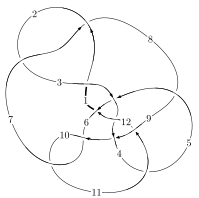
\includegraphics[width=112pt]{../../../GIT/diagram.site/Diagrams/png/2705_12n_0616.png}\\
\ \ \ A knot diagram\footnotemark}&
\allowdisplaybreaks
\textbf{Linearized knot diagam} \\
\cline{2-2}
 &
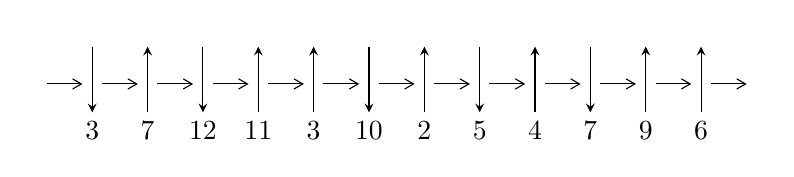
\begin{tikzpicture}[x=20pt, y=17pt]
	% nodes
	\node (C0) at (0, 0) {};
	\node (C1) at (1, 0) {};
	\node (C1U) at (1, +1) {};
	\node (C1D) at (1, -1) {3};

	\node (C2) at (2, 0) {};
	\node (C2U) at (2, +1) {};
	\node (C2D) at (2, -1) {7};

	\node (C3) at (3, 0) {};
	\node (C3U) at (3, +1) {};
	\node (C3D) at (3, -1) {12};

	\node (C4) at (4, 0) {};
	\node (C4U) at (4, +1) {};
	\node (C4D) at (4, -1) {11};

	\node (C5) at (5, 0) {};
	\node (C5U) at (5, +1) {};
	\node (C5D) at (5, -1) {3};

	\node (C6) at (6, 0) {};
	\node (C6U) at (6, +1) {};
	\node (C6D) at (6, -1) {10};

	\node (C7) at (7, 0) {};
	\node (C7U) at (7, +1) {};
	\node (C7D) at (7, -1) {2};

	\node (C8) at (8, 0) {};
	\node (C8U) at (8, +1) {};
	\node (C8D) at (8, -1) {5};

	\node (C9) at (9, 0) {};
	\node (C9U) at (9, +1) {};
	\node (C9D) at (9, -1) {4};

	\node (C10) at (10, 0) {};
	\node (C10U) at (10, +1) {};
	\node (C10D) at (10, -1) {7};

	\node (C11) at (11, 0) {};
	\node (C11U) at (11, +1) {};
	\node (C11D) at (11, -1) {9};

	\node (C12) at (12, 0) {};
	\node (C12U) at (12, +1) {};
	\node (C12D) at (12, -1) {6};
	\node (C13) at (13, 0) {};

	% arrows
	\draw[->,>={angle 60}]
	(C0) edge (C1) (C1) edge (C2) (C2) edge (C3) (C3) edge (C4) (C4) edge (C5) (C5) edge (C6) (C6) edge (C7) (C7) edge (C8) (C8) edge (C9) (C9) edge (C10) (C10) edge (C11) (C11) edge (C12) (C12) edge (C13) ;	\draw[->,>=stealth]
	(C1U) edge (C1D) (C2D) edge (C2U) (C3U) edge (C3D) (C4D) edge (C4U) (C5D) edge (C5U) (C6U) edge (C6D) (C7D) edge (C7U) (C8U) edge (C8D) (C9D) edge (C9U) (C10U) edge (C10D) (C11D) edge (C11U) (C12D) edge (C12U) ;
	\end{tikzpicture} \\
\hhline{~~} \\& 
\textbf{Solving Sequence} \\ \cline{2-2} 
 &
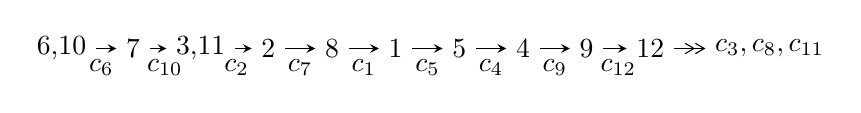
\begin{tikzpicture}[x=23pt, y=7pt]
	% node
	\node (A0) at (-1/8, 0) {6,10};
	\node (A1) at (1, 0) {7};
	\node (A2) at (33/16, 0) {3,11};
	\node (A3) at (25/8, 0) {2};
	\node (A4) at (33/8, 0) {8};
	\node (A5) at (41/8, 0) {1};
	\node (A6) at (49/8, 0) {5};
	\node (A7) at (57/8, 0) {4};
	\node (A8) at (65/8, 0) {9};
	\node (A9) at (73/8, 0) {12};
	\node (C1) at (1/2, -1) {$c_{6}$};
	\node (C2) at (3/2, -1) {$c_{10}$};
	\node (C3) at (21/8, -1) {$c_{2}$};
	\node (C4) at (29/8, -1) {$c_{7}$};
	\node (C5) at (37/8, -1) {$c_{1}$};
	\node (C6) at (45/8, -1) {$c_{5}$};
	\node (C7) at (53/8, -1) {$c_{4}$};
	\node (C8) at (61/8, -1) {$c_{9}$};
	\node (C9) at (69/8, -1) {$c_{12}$};
	\node (A10) at (11, 0) {$c_{3},c_{8},c_{11}$};

	% edge
	\draw[->,>=stealth]	
	(A0) edge (A1) (A1) edge (A2) (A2) edge (A3) (A3) edge (A4) (A4) edge (A5) (A5) edge (A6) (A6) edge (A7) (A7) edge (A8) (A8) edge (A9) ;
	\draw[->>,>={angle 60}]	
	(A9) edge (A10);
\end{tikzpicture} \\ 

\end{tabular} \\

\footnotetext{
The image of knot diagram is generated by the software ``\textbf{Draw programme}" developed by Andrew Bartholomew(\url{http://www.layer8.co.uk/maths/draw/index.htm\#Running-draw}), where we modified some parts for our purpose(\url{https://github.com/CATsTAILs/LinksPainter}).
}\phantom \\ \newline 
\centering \textbf{Ideals for irreducible components\footnotemark of $X_{\text{par}}$} 
 
\begin{align*}
I^u_{1}&=\langle 
3.55805\times10^{172} u^{61}-2.66340\times10^{172} u^{60}+\cdots+2.49043\times10^{174} b-1.12400\times10^{175},\\
\phantom{I^u_{1}}&\phantom{= \langle  }1.21069\times10^{173} u^{61}-1.41526\times10^{173} u^{60}+\cdots+2.24139\times10^{175} a-1.66162\times10^{174},\\
\phantom{I^u_{1}}&\phantom{= \langle  }u^{62}- u^{61}+\cdots-540 u+108\rangle \\
I^u_{2}&=\langle 
-4.69238\times10^{16} u^{29}-2.59707\times10^{16} u^{28}+\cdots+3.59633\times10^{16} b+1.14239\times10^{17},\\
\phantom{I^u_{2}}&\phantom{= \langle  }2.84054\times10^{17} u^{29}+2.41111\times10^{17} u^{28}+\cdots+3.59633\times10^{16} a-3.99453\times10^{17},\;u^{30}-8 u^{28}+\cdots+2 u+1\rangle \\
\\
\end{align*}
\raggedright * 2 irreducible components of $\dim_{\mathbb{C}}=0$, with total 92 representations.\\
\footnotetext{All coefficients of polynomials are rational numbers. But the coefficients are sometimes approximated in decimal forms when there is not enough margin.}
\newpage
\renewcommand{\arraystretch}{1}
\centering \section*{I. $I^u_{1}= \langle 3.56\times10^{172} u^{61}-2.66\times10^{172} u^{60}+\cdots+2.49\times10^{174} b-1.12\times10^{175},\;1.21\times10^{173} u^{61}-1.42\times10^{173} u^{60}+\cdots+2.24\times10^{175} a-1.66\times10^{174},\;u^{62}- u^{61}+\cdots-540 u+108 \rangle$}
\flushleft \textbf{(i) Arc colorings}\\
\begin{tabular}{m{7pt} m{180pt} m{7pt} m{180pt} }
\flushright $a_{6}=$&$\begin{pmatrix}1\\0\end{pmatrix}$ \\
\flushright $a_{10}=$&$\begin{pmatrix}0\\u\end{pmatrix}$ \\
\flushright $a_{7}=$&$\begin{pmatrix}1\\u^2\end{pmatrix}$ \\
\flushright $a_{3}=$&$\begin{pmatrix}-0.00540152 u^{61}+0.00631420 u^{60}+\cdots-10.9070 u+0.0741336\\-0.0142869 u^{61}+0.0106945 u^{60}+\cdots-11.8991 u+4.51328\end{pmatrix}$ \\
\flushright $a_{11}=$&$\begin{pmatrix}- u\\- u^3+u\end{pmatrix}$ \\
\flushright $a_{2}=$&$\begin{pmatrix}0.00910760 u^{61}-0.00500287 u^{60}+\cdots+2.06831 u-4.53772\\-0.0135155 u^{61}+0.00963239 u^{60}+\cdots-11.7423 u+4.16854\end{pmatrix}$ \\
\flushright $a_{8}=$&$\begin{pmatrix}-0.0102705 u^{61}+0.00570181 u^{60}+\cdots-15.8947 u+5.04760\\-0.00342408 u^{61}+0.00410364 u^{60}+\cdots-0.919576 u+2.86804\end{pmatrix}$ \\
\flushright $a_{1}=$&$\begin{pmatrix}0.00882729 u^{61}-0.00418130 u^{60}+\cdots+15.3641 u-4.48965\\0.0182728 u^{61}-0.0118352 u^{60}+\cdots+11.4934 u-4.66813\end{pmatrix}$ \\
\flushright $a_{5}=$&$\begin{pmatrix}0.0126898 u^{61}-0.00781485 u^{60}+\cdots+8.40923 u-4.07704\\0.00409918 u^{61}-0.00575768 u^{60}+\cdots+1.40699 u-3.26558\end{pmatrix}$ \\
\flushright $a_{4}=$&$\begin{pmatrix}0.0125680 u^{61}-0.00647401 u^{60}+\cdots+8.23390 u-3.71099\\0.00486562 u^{61}-0.00734645 u^{60}+\cdots+2.25375 u-3.76329\end{pmatrix}$ \\
\flushright $a_{9}=$&$\begin{pmatrix}-0.00661784 u^{61}+0.00354350 u^{60}+\cdots-6.75785 u+4.98454\\0.0172764 u^{61}-0.00999165 u^{60}+\cdots+14.4560 u-4.08059\end{pmatrix}$ \\
\flushright $a_{12}=$&$\begin{pmatrix}-0.00944546 u^{61}+0.00765391 u^{60}+\cdots+3.87066 u+0.178480\\0.0182728 u^{61}-0.0118352 u^{60}+\cdots+11.4934 u-4.66813\end{pmatrix}$\\&\end{tabular}
\flushleft \textbf{(ii) Obstruction class $= -1$}\\~\\
\flushleft \textbf{(iii) Cusp Shapes $= 0.0529669 u^{61}-0.0452256 u^{60}+\cdots+42.2033 u-18.0098$}\\~\\
\newpage\renewcommand{\arraystretch}{1}
\flushleft \textbf{(iv) u-Polynomials at the component}\newline \\
\begin{tabular}{m{50pt}|m{274pt}}
Crossings & \hspace{64pt}u-Polynomials at each crossing \\
\hline $$\begin{aligned}c_{1}\end{aligned}$$&$\begin{aligned}
&u^{62}+93 u^{61}+\cdots+2327471 u+1442401
\end{aligned}$\\
\hline $$\begin{aligned}c_{2},c_{7}\end{aligned}$$&$\begin{aligned}
&u^{62}- u^{61}+\cdots-7479 u+1201
\end{aligned}$\\
\hline $$\begin{aligned}c_{3}\end{aligned}$$&$\begin{aligned}
&u^{62}-5 u^{61}+\cdots-351 u+81
\end{aligned}$\\
\hline $$\begin{aligned}c_{4}\end{aligned}$$&$\begin{aligned}
&u^{62}+u^{61}+\cdots-29453 u+24019
\end{aligned}$\\
\hline $$\begin{aligned}c_{5}\end{aligned}$$&$\begin{aligned}
&u^{62}+45 u^{60}+\cdots-7939816 u+1967081
\end{aligned}$\\
\hline $$\begin{aligned}c_{6},c_{10}\end{aligned}$$&$\begin{aligned}
&u^{62}+u^{61}+\cdots+540 u+108
\end{aligned}$\\
\hline $$\begin{aligned}c_{8}\end{aligned}$$&$\begin{aligned}
&u^{62}+4 u^{61}+\cdots-17319366 u+37837071
\end{aligned}$\\
\hline $$\begin{aligned}c_{9}\end{aligned}$$&$\begin{aligned}
&u^{62}+2 u^{61}+\cdots+1506 u+313
\end{aligned}$\\
\hline $$\begin{aligned}c_{11}\end{aligned}$$&$\begin{aligned}
&u^{62}+3 u^{61}+\cdots+9 u+1
\end{aligned}$\\
\hline $$\begin{aligned}c_{12}\end{aligned}$$&$\begin{aligned}
&u^{62}+u^{61}+\cdots+40816 u+5087
\end{aligned}$\\
\hline
\end{tabular}\\~\\
\newpage\renewcommand{\arraystretch}{1}
\flushleft \textbf{(v) Riley Polynomials at the component}\newline \\
\begin{tabular}{m{50pt}|m{274pt}}
Crossings & \hspace{64pt}Riley Polynomials at each crossing \\
\hline $$\begin{aligned}c_{1}\end{aligned}$$&$\begin{aligned}
&y^{62}-227 y^{61}+\cdots+374501199567555 y+2080520644801
\end{aligned}$\\
\hline $$\begin{aligned}c_{2},c_{7}\end{aligned}$$&$\begin{aligned}
&y^{62}+93 y^{61}+\cdots+2327471 y+1442401
\end{aligned}$\\
\hline $$\begin{aligned}c_{3}\end{aligned}$$&$\begin{aligned}
&y^{62}+25 y^{61}+\cdots+101331 y+6561
\end{aligned}$\\
\hline $$\begin{aligned}c_{4}\end{aligned}$$&$\begin{aligned}
&y^{62}+27 y^{61}+\cdots+214913007 y+576912361
\end{aligned}$\\
\hline $$\begin{aligned}c_{5}\end{aligned}$$&$\begin{aligned}
&y^{62}+90 y^{61}+\cdots-46218775789508 y+3869407660561
\end{aligned}$\\
\hline $$\begin{aligned}c_{6},c_{10}\end{aligned}$$&$\begin{aligned}
&y^{62}-51 y^{61}+\cdots-56376 y+11664
\end{aligned}$\\
\hline $$\begin{aligned}c_{8}\end{aligned}$$&$\begin{aligned}
&y^{62}-60 y^{61}+\cdots+40273910932902534 y+1431643941859041
\end{aligned}$\\
\hline $$\begin{aligned}c_{9}\end{aligned}$$&$\begin{aligned}
&y^{62}+4 y^{61}+\cdots+269768 y+97969
\end{aligned}$\\
\hline $$\begin{aligned}c_{11}\end{aligned}$$&$\begin{aligned}
&y^{62}-5 y^{61}+\cdots-19 y+1
\end{aligned}$\\
\hline $$\begin{aligned}c_{12}\end{aligned}$$&$\begin{aligned}
&y^{62}+101 y^{61}+\cdots-990656780 y+25877569
\end{aligned}$\\
\hline
\end{tabular}\\~\\
\newpage\flushleft \textbf{(vi) Complex Volumes and Cusp Shapes}
$$\begin{array}{c|c|c}  
\text{Solutions to }I^u_{1}& \I (\text{vol} + \sqrt{-1}CS) & \text{Cusp shape}\\
 \hline 
\begin{aligned}
u &= -0.928426 + 0.274577 I \\
a &= -0.141263 - 0.866305 I \\
b &= -0.918957 - 0.595441 I\end{aligned}
 & \phantom{-}0.81276 + 2.95644 I & \phantom{-}8.56413 - 5.92863 I \\ \hline\begin{aligned}
u &= -0.928426 - 0.274577 I \\
a &= -0.141263 + 0.866305 I \\
b &= -0.918957 + 0.595441 I\end{aligned}
 & \phantom{-}0.81276 - 2.95644 I & \phantom{-}8.56413 + 5.92863 I \\ \hline\begin{aligned}
u &= -0.883961 + 0.394719 I \\
a &= \phantom{-}0.59269 - 1.64149 I \\
b &= -0.500699 - 0.932554 I\end{aligned}
 & -0.87581 + 4.78527 I & \phantom{-}0.6309 - 14.5936 I \\ \hline\begin{aligned}
u &= -0.883961 - 0.394719 I \\
a &= \phantom{-}0.59269 + 1.64149 I \\
b &= -0.500699 + 0.932554 I\end{aligned}
 & -0.87581 - 4.78527 I & \phantom{-}0.6309 + 14.5936 I \\ \hline\begin{aligned}
u &= \phantom{-}0.798892 + 0.328131 I \\
a &= -1.46380 - 0.42820 I \\
b &= -0.640242 - 0.054068 I\end{aligned}
 & -0.95457 - 1.51938 I & \phantom{-}1.17952 + 4.85265 I \\ \hline\begin{aligned}
u &= \phantom{-}0.798892 - 0.328131 I \\
a &= -1.46380 + 0.42820 I \\
b &= -0.640242 + 0.054068 I\end{aligned}
 & -0.95457 + 1.51938 I & \phantom{-}1.17952 - 4.85265 I \\ \hline\begin{aligned}
u &= \phantom{-}1.064810 + 0.545706 I \\
a &= -0.0830119 + 0.0387708 I \\
b &= \phantom{-}0.386898 + 0.525528 I\end{aligned}
 & -1.79842 - 1.83762 I & \phantom{-0.000000 } 0 \\ \hline\begin{aligned}
u &= \phantom{-}1.064810 - 0.545706 I \\
a &= -0.0830119 - 0.0387708 I \\
b &= \phantom{-}0.386898 - 0.525528 I\end{aligned}
 & -1.79842 + 1.83762 I & \phantom{-0.000000 } 0 \\ \hline\begin{aligned}
u &= \phantom{-}1.232990 + 0.083982 I \\
a &= \phantom{-}0.103400 - 0.171742 I \\
b &= -0.704160 + 0.181168 I\end{aligned}
 & -0.911910 + 0.560071 I & \phantom{-0.000000 } 0 \\ \hline\begin{aligned}
u &= \phantom{-}1.232990 - 0.083982 I \\
a &= \phantom{-}0.103400 + 0.171742 I \\
b &= -0.704160 - 0.181168 I\end{aligned}
 & -0.911910 - 0.560071 I & \phantom{-0.000000 } 0\\
 \hline 
 \end{array}$$\newpage$$\begin{array}{c|c|c}  
\text{Solutions to }I^u_{1}& \I (\text{vol} + \sqrt{-1}CS) & \text{Cusp shape}\\
 \hline 
\begin{aligned}
u &= \phantom{-}1.162130 + 0.432774 I \\
a &= \phantom{-}0.781400 + 0.862594 I \\
b &= -0.656170 + 0.829181 I\end{aligned}
 & -2.56521 - 5.62136 I & \phantom{-0.000000 } 0 \\ \hline\begin{aligned}
u &= \phantom{-}1.162130 - 0.432774 I \\
a &= \phantom{-}0.781400 - 0.862594 I \\
b &= -0.656170 - 0.829181 I\end{aligned}
 & -2.56521 + 5.62136 I & \phantom{-0.000000 } 0 \\ \hline\begin{aligned}
u &= -0.053502 + 1.258700 I \\
a &= -0.993543 + 0.161721 I \\
b &= \phantom{-}1.224160 + 0.468794 I\end{aligned}
 & \phantom{-}3.01979 - 1.86961 I & \phantom{-0.000000 } 0 \\ \hline\begin{aligned}
u &= -0.053502 - 1.258700 I \\
a &= -0.993543 - 0.161721 I \\
b &= \phantom{-}1.224160 - 0.468794 I\end{aligned}
 & \phantom{-}3.01979 + 1.86961 I & \phantom{-0.000000 } 0 \\ \hline\begin{aligned}
u &= \phantom{-}0.555763 + 0.420314 I \\
a &= -0.688240 + 0.980201 I \\
b &= -0.413944 - 0.903869 I\end{aligned}
 & -0.49204 + 1.99531 I & -0.82675 - 4.20883 I \\ \hline\begin{aligned}
u &= \phantom{-}0.555763 - 0.420314 I \\
a &= -0.688240 - 0.980201 I \\
b &= -0.413944 + 0.903869 I\end{aligned}
 & -0.49204 - 1.99531 I & -0.82675 + 4.20883 I \\ \hline\begin{aligned}
u &= \phantom{-}0.211720 + 1.290750 I \\
a &= \phantom{-}1.223300 - 0.047119 I \\
b &= -1.211470 - 0.325634 I\end{aligned}
 & \phantom{-}4.32311 - 2.81936 I & \phantom{-0.000000 } 0 \\ \hline\begin{aligned}
u &= \phantom{-}0.211720 - 1.290750 I \\
a &= \phantom{-}1.223300 + 0.047119 I \\
b &= -1.211470 + 0.325634 I\end{aligned}
 & \phantom{-}4.32311 + 2.81936 I & \phantom{-0.000000 } 0 \\ \hline\begin{aligned}
u &= -0.342685 + 1.277490 I \\
a &= -0.204814 + 0.198955 I \\
b &= \phantom{-}0.50743 - 1.99401 I\end{aligned}
 & -10.60230 + 1.13329 I & \phantom{-0.000000 } 0 \\ \hline\begin{aligned}
u &= -0.342685 - 1.277490 I \\
a &= -0.204814 - 0.198955 I \\
b &= \phantom{-}0.50743 + 1.99401 I\end{aligned}
 & -10.60230 - 1.13329 I & \phantom{-0.000000 } 0\\
 \hline 
 \end{array}$$\newpage$$\begin{array}{c|c|c}  
\text{Solutions to }I^u_{1}& \I (\text{vol} + \sqrt{-1}CS) & \text{Cusp shape}\\
 \hline 
\begin{aligned}
u &= -0.614267 + 0.283569 I \\
a &= -1.021740 - 0.249635 I \\
b &= -0.711770 + 0.261415 I\end{aligned}
 & \phantom{-}1.381510 - 0.110117 I & \phantom{-}9.95847 - 1.16431 I \\ \hline\begin{aligned}
u &= -0.614267 - 0.283569 I \\
a &= -1.021740 + 0.249635 I \\
b &= -0.711770 - 0.261415 I\end{aligned}
 & \phantom{-}1.381510 + 0.110117 I & \phantom{-}9.95847 + 1.16431 I \\ \hline\begin{aligned}
u &= \phantom{-}1.188520 + 0.601200 I \\
a &= -0.477089 - 0.246417 I \\
b &= \phantom{-}0.493192 + 0.235501 I\end{aligned}
 & -2.66613 - 1.84132 I & \phantom{-0.000000 } 0 \\ \hline\begin{aligned}
u &= \phantom{-}1.188520 - 0.601200 I \\
a &= -0.477089 + 0.246417 I \\
b &= \phantom{-}0.493192 - 0.235501 I\end{aligned}
 & -2.66613 + 1.84132 I & \phantom{-0.000000 } 0 \\ \hline\begin{aligned}
u &= -0.568370 + 0.290816 I \\
a &= -1.077140 + 0.714898 I \\
b &= \phantom{-}0.031563 - 1.189600 I\end{aligned}
 & -9.40415 + 0.96502 I & -3.47084 - 7.40489 I \\ \hline\begin{aligned}
u &= -0.568370 - 0.290816 I \\
a &= -1.077140 - 0.714898 I \\
b &= \phantom{-}0.031563 + 1.189600 I\end{aligned}
 & -9.40415 - 0.96502 I & -3.47084 + 7.40489 I \\ \hline\begin{aligned}
u &= \phantom{-}0.173116 + 0.612853 I \\
a &= -1.97761 + 1.41609 I \\
b &= \phantom{-}0.761201 - 0.088010 I\end{aligned}
 & \phantom{-}3.33244 - 2.13366 I & \phantom{-}9.28813 + 3.63241 I \\ \hline\begin{aligned}
u &= \phantom{-}0.173116 - 0.612853 I \\
a &= -1.97761 - 1.41609 I \\
b &= \phantom{-}0.761201 + 0.088010 I\end{aligned}
 & \phantom{-}3.33244 + 2.13366 I & \phantom{-}9.28813 - 3.63241 I \\ \hline\begin{aligned}
u &= -1.237450 + 0.584054 I \\
a &= \phantom{-}0.412477 + 0.156333 I \\
b &= \phantom{-}0.857350 - 0.607671 I\end{aligned}
 & -0.60518 + 7.63571 I & \phantom{-0.000000 } 0 \\ \hline\begin{aligned}
u &= -1.237450 - 0.584054 I \\
a &= \phantom{-}0.412477 - 0.156333 I \\
b &= \phantom{-}0.857350 + 0.607671 I\end{aligned}
 & -0.60518 - 7.63571 I & \phantom{-0.000000 } 0\\
 \hline 
 \end{array}$$\newpage$$\begin{array}{c|c|c}  
\text{Solutions to }I^u_{1}& \I (\text{vol} + \sqrt{-1}CS) & \text{Cusp shape}\\
 \hline 
\begin{aligned}
u &= \phantom{-}1.337770 + 0.289922 I \\
a &= -0.616546 - 1.234550 I \\
b &= -0.84829 - 1.37346 I\end{aligned}
 & -2.91445 - 1.23024 I & \phantom{-0.000000 } 0 \\ \hline\begin{aligned}
u &= \phantom{-}1.337770 - 0.289922 I \\
a &= -0.616546 + 1.234550 I \\
b &= -0.84829 + 1.37346 I\end{aligned}
 & -2.91445 + 1.23024 I & \phantom{-0.000000 } 0 \\ \hline\begin{aligned}
u &= \phantom{-}0.528204 + 0.322278 I \\
a &= -1.136860 + 0.092169 I \\
b &= -0.300012 + 0.378008 I\end{aligned}
 & -0.80326 - 1.53767 I & -1.79348 + 5.24850 I \\ \hline\begin{aligned}
u &= \phantom{-}0.528204 - 0.322278 I \\
a &= -1.136860 - 0.092169 I \\
b &= -0.300012 - 0.378008 I\end{aligned}
 & -0.80326 + 1.53767 I & -1.79348 - 5.24850 I \\ \hline\begin{aligned}
u &= \phantom{-}1.397880 + 0.097398 I \\
a &= \phantom{-}0.10957 + 2.12503 I \\
b &= -0.41120 + 2.32836 I\end{aligned}
 & -9.86019 - 4.97411 I & \phantom{-0.000000 } 0 \\ \hline\begin{aligned}
u &= \phantom{-}1.397880 - 0.097398 I \\
a &= \phantom{-}0.10957 - 2.12503 I \\
b &= -0.41120 - 2.32836 I\end{aligned}
 & -9.86019 + 4.97411 I & \phantom{-0.000000 } 0 \\ \hline\begin{aligned}
u &= -1.41670 + 0.03978 I \\
a &= \phantom{-}0.056166 + 1.051810 I \\
b &= \phantom{-}0.96710 + 1.03620 I\end{aligned}
 & -6.57035 - 1.95796 I & \phantom{-0.000000 } 0 \\ \hline\begin{aligned}
u &= -1.41670 - 0.03978 I \\
a &= \phantom{-}0.056166 - 1.051810 I \\
b &= \phantom{-}0.96710 - 1.03620 I\end{aligned}
 & -6.57035 + 1.95796 I & \phantom{-0.000000 } 0 \\ \hline\begin{aligned}
u &= -1.42483 + 0.05605 I \\
a &= -0.14962 + 1.95097 I \\
b &= -0.32405 + 1.90177 I\end{aligned}
 & -13.12830 + 0.25112 I & \phantom{-0.000000 } 0 \\ \hline\begin{aligned}
u &= -1.42483 - 0.05605 I \\
a &= -0.14962 - 1.95097 I \\
b &= -0.32405 - 1.90177 I\end{aligned}
 & -13.12830 - 0.25112 I & \phantom{-0.000000 } 0\\
 \hline 
 \end{array}$$\newpage$$\begin{array}{c|c|c}  
\text{Solutions to }I^u_{1}& \I (\text{vol} + \sqrt{-1}CS) & \text{Cusp shape}\\
 \hline 
\begin{aligned}
u &= -0.138714 + 0.382151 I \\
a &= -1.028670 - 0.003428 I \\
b &= -0.405698 + 0.592213 I\end{aligned}
 & \phantom{-}0.56906 - 1.80805 I & \phantom{-}2.62914 + 3.42135 I \\ \hline\begin{aligned}
u &= -0.138714 - 0.382151 I \\
a &= -1.028670 + 0.003428 I \\
b &= -0.405698 - 0.592213 I\end{aligned}
 & \phantom{-}0.56906 + 1.80805 I & \phantom{-}2.62914 - 3.42135 I \\ \hline\begin{aligned}
u &= -1.59777 + 0.24654 I \\
a &= -0.140434 + 0.972924 I \\
b &= -0.81650 + 1.30662 I\end{aligned}
 & -3.14029 + 8.05378 I & \phantom{-0.000000 } 0 \\ \hline\begin{aligned}
u &= -1.59777 - 0.24654 I \\
a &= -0.140434 - 0.972924 I \\
b &= -0.81650 - 1.30662 I\end{aligned}
 & -3.14029 - 8.05378 I & \phantom{-0.000000 } 0 \\ \hline\begin{aligned}
u &= \phantom{-}1.53281 + 0.53294 I \\
a &= \phantom{-}0.81860 + 1.41695 I \\
b &= -0.23778 + 2.39126 I\end{aligned}
 & -16.3568 - 7.4045 I & \phantom{-0.000000 } 0 \\ \hline\begin{aligned}
u &= \phantom{-}1.53281 - 0.53294 I \\
a &= \phantom{-}0.81860 - 1.41695 I \\
b &= -0.23778 - 2.39126 I\end{aligned}
 & -16.3568 + 7.4045 I & \phantom{-0.000000 } 0 \\ \hline\begin{aligned}
u &= \phantom{-}0.330694 + 0.108076 I \\
a &= -1.128190 - 0.118541 I \\
b &= -0.21404 - 1.58285 I\end{aligned}
 & -5.82473 + 4.09311 I & -7.36144 + 5.13793 I \\ \hline\begin{aligned}
u &= \phantom{-}0.330694 - 0.108076 I \\
a &= -1.128190 + 0.118541 I \\
b &= -0.21404 + 1.58285 I\end{aligned}
 & -5.82473 - 4.09311 I & -7.36144 - 5.13793 I \\ \hline\begin{aligned}
u &= -0.053813 + 0.324295 I \\
a &= -3.15267 - 5.18917 I \\
b &= \phantom{-}0.633235 - 0.211555 I\end{aligned}
 & \phantom{-}3.29821 - 6.08310 I & \phantom{-}10.9240 + 9.4569 I \\ \hline\begin{aligned}
u &= -0.053813 - 0.324295 I \\
a &= -3.15267 + 5.18917 I \\
b &= \phantom{-}0.633235 + 0.211555 I\end{aligned}
 & \phantom{-}3.29821 + 6.08310 I & \phantom{-}10.9240 - 9.4569 I\\
 \hline 
 \end{array}$$\newpage$$\begin{array}{c|c|c}  
\text{Solutions to }I^u_{1}& \I (\text{vol} + \sqrt{-1}CS) & \text{Cusp shape}\\
 \hline 
\begin{aligned}
u &= \phantom{-}0.06429 + 1.70451 I \\
a &= -0.034729 - 0.171847 I \\
b &= \phantom{-}0.17523 + 2.51987 I\end{aligned}
 & -8.83971 + 7.11017 I & \phantom{-0.000000 } 0 \\ \hline\begin{aligned}
u &= \phantom{-}0.06429 - 1.70451 I \\
a &= -0.034729 + 0.171847 I \\
b &= \phantom{-}0.17523 - 2.51987 I\end{aligned}
 & -8.83971 - 7.11017 I & \phantom{-0.000000 } 0 \\ \hline\begin{aligned}
u &= -1.51413 + 0.82312 I \\
a &= -0.89512 + 1.12015 I \\
b &= \phantom{-}1.05248 + 2.06010 I\end{aligned}
 & -14.0247 + 6.7818 I & \phantom{-0.000000 } 0 \\ \hline\begin{aligned}
u &= -1.51413 - 0.82312 I \\
a &= -0.89512 - 1.12015 I \\
b &= \phantom{-}1.05248 - 2.06010 I\end{aligned}
 & -14.0247 - 6.7818 I & \phantom{-0.000000 } 0 \\ \hline\begin{aligned}
u &= \phantom{-}1.74221 + 0.14569 I \\
a &= \phantom{-}0.225196 - 0.756516 I \\
b &= \phantom{-}1.81283 - 1.03004 I\end{aligned}
 & -4.56049 - 4.34139 I & \phantom{-0.000000 } 0 \\ \hline\begin{aligned}
u &= \phantom{-}1.74221 - 0.14569 I \\
a &= \phantom{-}0.225196 + 0.756516 I \\
b &= \phantom{-}1.81283 + 1.03004 I\end{aligned}
 & -4.56049 + 4.34139 I & \phantom{-0.000000 } 0 \\ \hline\begin{aligned}
u &= \phantom{-}1.58884 + 0.74366 I \\
a &= -0.81842 - 1.19718 I \\
b &= \phantom{-}0.81340 - 2.28442 I\end{aligned}
 & -13.7046 - 15.4840 I & \phantom{-0.000000 } 0 \\ \hline\begin{aligned}
u &= \phantom{-}1.58884 - 0.74366 I \\
a &= -0.81842 + 1.19718 I \\
b &= \phantom{-}0.81340 + 2.28442 I\end{aligned}
 & -13.7046 + 15.4840 I & \phantom{-0.000000 } 0 \\ \hline\begin{aligned}
u &= -1.75665 + 0.11101 I \\
a &= \phantom{-}0.12382 - 1.45778 I \\
b &= \phantom{-}0.12632 - 2.39437 I\end{aligned}
 & -14.1931 + 4.3228 I & \phantom{-0.000000 } 0 \\ \hline\begin{aligned}
u &= -1.75665 - 0.11101 I \\
a &= \phantom{-}0.12382 + 1.45778 I \\
b &= \phantom{-}0.12632 + 2.39437 I\end{aligned}
 & -14.1931 - 4.3228 I & \phantom{-0.000000 } 0\\
 \hline 
 \end{array}$$\newpage$$\begin{array}{c|c|c}  
\text{Solutions to }I^u_{1}& \I (\text{vol} + \sqrt{-1}CS) & \text{Cusp shape}\\
 \hline 
\begin{aligned}
u &= -1.87938 + 0.62453 I \\
a &= \phantom{-}0.532884 - 1.112330 I \\
b &= -0.52742 - 2.72829 I\end{aligned}
 & -15.0495 + 1.7796 I & \phantom{-0.000000 } 0 \\ \hline\begin{aligned}
u &= -1.87938 - 0.62453 I \\
a &= \phantom{-}0.532884 + 1.112330 I \\
b &= -0.52742 + 2.72829 I\end{aligned}
 & -15.0495 - 1.7796 I & \phantom{-0.000000 } 0\\
 \hline 
 \end{array}$$\newpage\newpage\renewcommand{\arraystretch}{1}
\centering \section*{II. $I^u_{2}= \langle -4.69\times10^{16} u^{29}-2.60\times10^{16} u^{28}+\cdots+3.60\times10^{16} b+1.14\times10^{17},\;2.84\times10^{17} u^{29}+2.41\times10^{17} u^{28}+\cdots+3.60\times10^{16} a-3.99\times10^{17},\;u^{30}-8 u^{28}+\cdots+2 u+1 \rangle$}
\flushleft \textbf{(i) Arc colorings}\\
\begin{tabular}{m{7pt} m{180pt} m{7pt} m{180pt} }
\flushright $a_{6}=$&$\begin{pmatrix}1\\0\end{pmatrix}$ \\
\flushright $a_{10}=$&$\begin{pmatrix}0\\u\end{pmatrix}$ \\
\flushright $a_{7}=$&$\begin{pmatrix}1\\u^2\end{pmatrix}$ \\
\flushright $a_{3}=$&$\begin{pmatrix}-7.89844 u^{29}-6.70438 u^{28}+\cdots+46.1262 u+11.1073\\1.30477 u^{29}+0.722144 u^{28}+\cdots-12.6546 u-3.17653\end{pmatrix}$ \\
\flushright $a_{11}=$&$\begin{pmatrix}- u\\- u^3+u\end{pmatrix}$ \\
\flushright $a_{2}=$&$\begin{pmatrix}-11.9788 u^{29}-10.9744 u^{28}+\cdots+80.0880 u+20.9882\\0.00854127 u^{29}-0.937725 u^{28}+\cdots-0.0341923 u+1.09346\end{pmatrix}$ \\
\flushright $a_{8}=$&$\begin{pmatrix}19.2699 u^{29}+21.0285 u^{28}+\cdots-171.610 u-55.6470\\0.986098 u^{29}+3.09570 u^{28}+\cdots-23.0758 u-8.58984\end{pmatrix}$ \\
\flushright $a_{1}=$&$\begin{pmatrix}-19.6132 u^{29}-21.5167 u^{28}+\cdots+176.130 u+56.8875\\-3.35827 u^{29}-3.80005 u^{28}+\cdots+28.1757 u+8.57614\end{pmatrix}$ \\
\flushright $a_{5}=$&$\begin{pmatrix}-4.33768 u^{29}-1.92583 u^{28}+\cdots+27.6131 u+8.41369\\-1.40261 u^{29}-1.92358 u^{28}+\cdots+17.1060 u+5.96332\end{pmatrix}$ \\
\flushright $a_{4}=$&$\begin{pmatrix}-2.40167 u^{29}-1.05482 u^{28}+\cdots+17.1659 u+5.23135\\-2.77770 u^{29}-2.46020 u^{28}+\cdots+23.8751 u+8.27464\end{pmatrix}$ \\
\flushright $a_{9}=$&$\begin{pmatrix}4.79433 u^{29}+4.95182 u^{28}+\cdots-45.5614 u-11.8368\\4.33349 u^{29}+4.31110 u^{28}+\cdots-35.8661 u-9.73763\end{pmatrix}$ \\
\flushright $a_{12}=$&$\begin{pmatrix}-16.2549 u^{29}-17.7167 u^{28}+\cdots+147.955 u+48.3114\\-3.35827 u^{29}-3.80005 u^{28}+\cdots+28.1757 u+8.57614\end{pmatrix}$\\&\end{tabular}
\flushleft \textbf{(ii) Obstruction class $= 1$}\\~\\
\flushleft \textbf{(iii) Cusp Shapes $= -\frac{5213218321058946}{35963279984144951} u^{29}-\frac{204199795425121514}{35963279984144951} u^{28}+\cdots+\frac{553381217539182497}{35963279984144951} u+\frac{8083989187387400}{35963279984144951}$}\\~\\
\newpage\renewcommand{\arraystretch}{1}
\flushleft \textbf{(iv) u-Polynomials at the component}\newline \\
\begin{tabular}{m{50pt}|m{274pt}}
Crossings & \hspace{64pt}u-Polynomials at each crossing \\
\hline $$\begin{aligned}c_{1}\end{aligned}$$&$\begin{aligned}
&u^{30}-32 u^{29}+\cdots-27 u+1
\end{aligned}$\\
\hline $$\begin{aligned}c_{2}\end{aligned}$$&$\begin{aligned}
&u^{30}+16 u^{28}+\cdots-3 u+1
\end{aligned}$\\
\hline $$\begin{aligned}c_{3}\end{aligned}$$&$\begin{aligned}
&u^{30}+8 u^{29}+\cdots+23 u+11
\end{aligned}$\\
\hline $$\begin{aligned}c_{4}\end{aligned}$$&$\begin{aligned}
&u^{30}+4 u^{29}+\cdots+3 u+1
\end{aligned}$\\
\hline $$\begin{aligned}c_{5}\end{aligned}$$&$\begin{aligned}
&u^{30}-5 u^{29}+\cdots-6 u^2+1
\end{aligned}$\\
\hline $$\begin{aligned}c_{6}\end{aligned}$$&$\begin{aligned}
&u^{30}-8 u^{28}+\cdots+2 u+1
\end{aligned}$\\
\hline $$\begin{aligned}c_{7}\end{aligned}$$&$\begin{aligned}
&u^{30}+16 u^{28}+\cdots+3 u+1
\end{aligned}$\\
\hline $$\begin{aligned}c_{8}\end{aligned}$$&$\begin{aligned}
&u^{30}+u^{29}+\cdots+12 u+1
\end{aligned}$\\
\hline $$\begin{aligned}c_{9}\end{aligned}$$&$\begin{aligned}
&u^{30}+u^{29}+\cdots+6 u^2+1
\end{aligned}$\\
\hline $$\begin{aligned}c_{10}\end{aligned}$$&$\begin{aligned}
&u^{30}-8 u^{28}+\cdots-2 u+1
\end{aligned}$\\
\hline $$\begin{aligned}c_{11}\end{aligned}$$&$\begin{aligned}
&u^{30}-6 u^{29}+\cdots-3 u+1
\end{aligned}$\\
\hline $$\begin{aligned}c_{12}\end{aligned}$$&$\begin{aligned}
&u^{30}+16 u^{28}+\cdots+148 u+73
\end{aligned}$\\
\hline
\end{tabular}\\~\\
\newpage\renewcommand{\arraystretch}{1}
\flushleft \textbf{(v) Riley Polynomials at the component}\newline \\
\begin{tabular}{m{50pt}|m{274pt}}
Crossings & \hspace{64pt}Riley Polynomials at each crossing \\
\hline $$\begin{aligned}c_{1}\end{aligned}$$&$\begin{aligned}
&y^{30}-48 y^{29}+\cdots+267 y+1
\end{aligned}$\\
\hline $$\begin{aligned}c_{2},c_{7}\end{aligned}$$&$\begin{aligned}
&y^{30}+32 y^{29}+\cdots+27 y+1
\end{aligned}$\\
\hline $$\begin{aligned}c_{3}\end{aligned}$$&$\begin{aligned}
&y^{30}+16 y^{29}+\cdots+2199 y+121
\end{aligned}$\\
\hline $$\begin{aligned}c_{4}\end{aligned}$$&$\begin{aligned}
&y^{30}-2 y^{29}+\cdots+15 y+1
\end{aligned}$\\
\hline $$\begin{aligned}c_{5}\end{aligned}$$&$\begin{aligned}
&y^{30}+9 y^{29}+\cdots-12 y+1
\end{aligned}$\\
\hline $$\begin{aligned}c_{6},c_{10}\end{aligned}$$&$\begin{aligned}
&y^{30}-16 y^{29}+\cdots-18 y+1
\end{aligned}$\\
\hline $$\begin{aligned}c_{8}\end{aligned}$$&$\begin{aligned}
&y^{30}-9 y^{29}+\cdots+154 y+1
\end{aligned}$\\
\hline $$\begin{aligned}c_{9}\end{aligned}$$&$\begin{aligned}
&y^{30}-5 y^{29}+\cdots+12 y+1
\end{aligned}$\\
\hline $$\begin{aligned}c_{11}\end{aligned}$$&$\begin{aligned}
&y^{30}-6 y^{29}+\cdots-11 y+1
\end{aligned}$\\
\hline $$\begin{aligned}c_{12}\end{aligned}$$&$\begin{aligned}
&y^{30}+32 y^{29}+\cdots-588 y+5329
\end{aligned}$\\
\hline
\end{tabular}\\~\\
\newpage\flushleft \textbf{(vi) Complex Volumes and Cusp Shapes}
$$\begin{array}{c|c|c}  
\text{Solutions to }I^u_{2}& \I (\text{vol} + \sqrt{-1}CS) & \text{Cusp shape}\\
 \hline 
\begin{aligned}
u &= -0.875224 + 0.412321 I \\
a &= \phantom{-}1.69841 - 0.60554 I \\
b &= \phantom{-}0.760440 - 0.576623 I\end{aligned}
 & -0.932767 + 0.879726 I & \phantom{-}3.02133 + 5.92289 I \\ \hline\begin{aligned}
u &= -0.875224 - 0.412321 I \\
a &= \phantom{-}1.69841 + 0.60554 I \\
b &= \phantom{-}0.760440 + 0.576623 I\end{aligned}
 & -0.932767 - 0.879726 I & \phantom{-}3.02133 - 5.92289 I \\ \hline\begin{aligned}
u &= -0.942420 + 0.425846 I \\
a &= \phantom{-}0.990477 + 0.135569 I \\
b &= \phantom{-}0.667510 + 0.309330 I\end{aligned}
 & -1.20958 + 2.51761 I & \phantom{-}3.24397 - 8.62261 I \\ \hline\begin{aligned}
u &= -0.942420 - 0.425846 I \\
a &= \phantom{-}0.990477 - 0.135569 I \\
b &= \phantom{-}0.667510 - 0.309330 I\end{aligned}
 & -1.20958 - 2.51761 I & \phantom{-}3.24397 + 8.62261 I \\ \hline\begin{aligned}
u &= \phantom{-}0.918962 + 0.185501 I \\
a &= \phantom{-}0.772753 - 0.368979 I \\
b &= \phantom{-}0.980426 + 0.543348 I\end{aligned}
 & \phantom{-}0.449422 + 0.992006 I & \phantom{-}4.91900 - 1.24662 I \\ \hline\begin{aligned}
u &= \phantom{-}0.918962 - 0.185501 I \\
a &= \phantom{-}0.772753 + 0.368979 I \\
b &= \phantom{-}0.980426 - 0.543348 I\end{aligned}
 & \phantom{-}0.449422 - 0.992006 I & \phantom{-}4.91900 + 1.24662 I \\ \hline\begin{aligned}
u &= \phantom{-}0.805987 + 0.473388 I \\
a &= -1.14949 - 1.16426 I \\
b &= \phantom{-}0.472421 - 0.931467 I\end{aligned}
 & -1.04141 - 4.12353 I & -1.85641 + 2.83850 I \\ \hline\begin{aligned}
u &= \phantom{-}0.805987 - 0.473388 I \\
a &= -1.14949 + 1.16426 I \\
b &= \phantom{-}0.472421 + 0.931467 I\end{aligned}
 & -1.04141 + 4.12353 I & -1.85641 - 2.83850 I \\ \hline\begin{aligned}
u &= \phantom{-}1.030030 + 0.445576 I \\
a &= -0.224858 - 1.133130 I \\
b &= \phantom{-}0.752856 - 0.363100 I\end{aligned}
 & -0.50274 - 3.54177 I & \phantom{-}2.42929 + 4.86648 I \\ \hline\begin{aligned}
u &= \phantom{-}1.030030 - 0.445576 I \\
a &= -0.224858 + 1.133130 I \\
b &= \phantom{-}0.752856 + 0.363100 I\end{aligned}
 & -0.50274 + 3.54177 I & \phantom{-}2.42929 - 4.86648 I\\
 \hline 
 \end{array}$$\newpage$$\begin{array}{c|c|c}  
\text{Solutions to }I^u_{2}& \I (\text{vol} + \sqrt{-1}CS) & \text{Cusp shape}\\
 \hline 
\begin{aligned}
u &= \phantom{-}1.101300 + 0.335368 I \\
a &= \phantom{-}0.718236 + 0.312049 I \\
b &= \phantom{-}0.365568 + 0.668549 I\end{aligned}
 & -2.43063 + 0.67941 I & -4.10126 - 2.36820 I \\ \hline\begin{aligned}
u &= \phantom{-}1.101300 - 0.335368 I \\
a &= \phantom{-}0.718236 - 0.312049 I \\
b &= \phantom{-}0.365568 - 0.668549 I\end{aligned}
 & -2.43063 - 0.67941 I & -4.10126 + 2.36820 I \\ \hline\begin{aligned}
u &= -0.637051 + 0.475657 I \\
a &= -0.641785 + 0.810694 I \\
b &= \phantom{-}0.371089 - 1.189360 I\end{aligned}
 & -9.15677 + 0.14682 I & \phantom{-}1.19258 + 1.36386 I \\ \hline\begin{aligned}
u &= -0.637051 - 0.475657 I \\
a &= -0.641785 - 0.810694 I \\
b &= \phantom{-}0.371089 + 1.189360 I\end{aligned}
 & -9.15677 - 0.14682 I & \phantom{-}1.19258 - 1.36386 I \\ \hline\begin{aligned}
u &= -1.198170 + 0.492756 I \\
a &= -0.389462 + 0.514253 I \\
b &= -0.429522 + 0.342584 I\end{aligned}
 & -0.28781 + 8.86990 I & \phantom{-}2.50133 - 9.25007 I \\ \hline\begin{aligned}
u &= -1.198170 - 0.492756 I \\
a &= -0.389462 - 0.514253 I \\
b &= -0.429522 - 0.342584 I\end{aligned}
 & -0.28781 - 8.86990 I & \phantom{-}2.50133 + 9.25007 I \\ \hline\begin{aligned}
u &= \phantom{-}0.347894 + 1.261540 I \\
a &= -1.145370 - 0.093955 I \\
b &= \phantom{-}1.46537 + 0.16374 I\end{aligned}
 & \phantom{-}2.87728 - 1.15731 I & -0.12131 - 4.65886 I \\ \hline\begin{aligned}
u &= \phantom{-}0.347894 - 1.261540 I \\
a &= -1.145370 + 0.093955 I \\
b &= \phantom{-}1.46537 - 0.16374 I\end{aligned}
 & \phantom{-}2.87728 + 1.15731 I & -0.12131 + 4.65886 I \\ \hline\begin{aligned}
u &= -0.582042 + 0.114441 I \\
a &= -3.71699 + 1.44960 I \\
b &= -0.518015 + 0.023656 I\end{aligned}
 & \phantom{-}2.80413 - 5.94257 I & -4.38802 + 4.41854 I \\ \hline\begin{aligned}
u &= -0.582042 - 0.114441 I \\
a &= -3.71699 - 1.44960 I \\
b &= -0.518015 - 0.023656 I\end{aligned}
 & \phantom{-}2.80413 + 5.94257 I & -4.38802 - 4.41854 I\\
 \hline 
 \end{array}$$\newpage$$\begin{array}{c|c|c}  
\text{Solutions to }I^u_{2}& \I (\text{vol} + \sqrt{-1}CS) & \text{Cusp shape}\\
 \hline 
\begin{aligned}
u &= \phantom{-}0.592085 + 0.032840 I \\
a &= -3.11419 - 1.27073 I \\
b &= -0.431358 + 0.454461 I\end{aligned}
 & \phantom{-}2.54811 - 1.76721 I & -0.0133359 - 0.0791266 I \\ \hline\begin{aligned}
u &= \phantom{-}0.592085 - 0.032840 I \\
a &= -3.11419 + 1.27073 I \\
b &= -0.431358 - 0.454461 I\end{aligned}
 & \phantom{-}2.54811 + 1.76721 I & -0.0133359 + 0.0791266 I \\ \hline\begin{aligned}
u &= -0.03393 + 1.43301 I \\
a &= \phantom{-}0.954956 - 0.213579 I \\
b &= -1.060600 - 0.576962 I\end{aligned}
 & \phantom{-}4.04859 - 3.36586 I & \phantom{-}2.59994 + 9.05520 I \\ \hline\begin{aligned}
u &= -0.03393 - 1.43301 I \\
a &= \phantom{-}0.954956 + 0.213579 I \\
b &= -1.060600 + 0.576962 I\end{aligned}
 & \phantom{-}4.04859 + 3.36586 I & \phantom{-}2.59994 - 9.05520 I \\ \hline\begin{aligned}
u &= -0.289164 + 0.364349 I \\
a &= -0.762478 + 0.282994 I \\
b &= \phantom{-}0.13710 + 1.64032 I\end{aligned}
 & -5.61406 + 4.42294 I & \phantom{-}3.80460 - 11.65991 I \\ \hline\begin{aligned}
u &= -0.289164 - 0.364349 I \\
a &= -0.762478 - 0.282994 I \\
b &= \phantom{-}0.13710 - 1.64032 I\end{aligned}
 & -5.61406 - 4.42294 I & \phantom{-}3.80460 + 11.65991 I \\ \hline\begin{aligned}
u &= \phantom{-}1.50756 + 0.48121 I \\
a &= \phantom{-}0.300988 + 0.564457 I \\
b &= -1.175620 + 0.291973 I\end{aligned}
 & -2.12714 - 3.25888 I & \phantom{-}0.91150 + 4.03136 I \\ \hline\begin{aligned}
u &= \phantom{-}1.50756 - 0.48121 I \\
a &= \phantom{-}0.300988 - 0.564457 I \\
b &= -1.175620 - 0.291973 I\end{aligned}
 & -2.12714 + 3.25888 I & \phantom{-}0.91150 - 4.03136 I \\ \hline\begin{aligned}
u &= -1.74582 + 0.25668 I \\
a &= -0.29120 + 1.43523 I \\
b &= \phantom{-}0.14233 + 2.41540 I\end{aligned}
 & -14.0986 + 3.6495 I & \phantom{-0.000000 } 0 \\ \hline\begin{aligned}
u &= -1.74582 - 0.25668 I \\
a &= -0.29120 - 1.43523 I \\
b &= \phantom{-}0.14233 - 2.41540 I\end{aligned}
 & -14.0986 - 3.6495 I & \phantom{-0.000000 } 0\\
 \hline 
 \end{array}$$\newpage
\newpage\renewcommand{\arraystretch}{1}
\centering \section*{ III. u-Polynomials}
\begin{tabular}{m{50pt}|m{274pt}}
Crossings & \hspace{64pt}u-Polynomials at each crossing \\
\hline $$\begin{aligned}c_{1}\end{aligned}$$&$\begin{aligned}
&(u^{30}-32 u^{29}+\cdots-27 u+1)\\
&\cdot(u^{62}+93 u^{61}+\cdots+2327471 u+1442401)
\end{aligned}$\\
\hline $$\begin{aligned}c_{2}\end{aligned}$$&$\begin{aligned}
&(u^{30}+16 u^{28}+\cdots-3 u+1)(u^{62}- u^{61}+\cdots-7479 u+1201)
\end{aligned}$\\
\hline $$\begin{aligned}c_{3}\end{aligned}$$&$\begin{aligned}
&(u^{30}+8 u^{29}+\cdots+23 u+11)(u^{62}-5 u^{61}+\cdots-351 u+81)
\end{aligned}$\\
\hline $$\begin{aligned}c_{4}\end{aligned}$$&$\begin{aligned}
&(u^{30}+4 u^{29}+\cdots+3 u+1)(u^{62}+u^{61}+\cdots-29453 u+24019)
\end{aligned}$\\
\hline $$\begin{aligned}c_{5}\end{aligned}$$&$\begin{aligned}
&(u^{30}-5 u^{29}+\cdots-6 u^2+1)(u^{62}+45 u^{60}+\cdots-7939816 u+1967081)
\end{aligned}$\\
\hline $$\begin{aligned}c_{6}\end{aligned}$$&$\begin{aligned}
&(u^{30}-8 u^{28}+\cdots+2 u+1)(u^{62}+u^{61}+\cdots+540 u+108)
\end{aligned}$\\
\hline $$\begin{aligned}c_{7}\end{aligned}$$&$\begin{aligned}
&(u^{30}+16 u^{28}+\cdots+3 u+1)(u^{62}- u^{61}+\cdots-7479 u+1201)
\end{aligned}$\\
\hline $$\begin{aligned}c_{8}\end{aligned}$$&$\begin{aligned}
&(u^{30}+u^{29}+\cdots+12 u+1)\\
&\cdot(u^{62}+4 u^{61}+\cdots-17319366 u+37837071)
\end{aligned}$\\
\hline $$\begin{aligned}c_{9}\end{aligned}$$&$\begin{aligned}
&(u^{30}+u^{29}+\cdots+6 u^2+1)(u^{62}+2 u^{61}+\cdots+1506 u+313)
\end{aligned}$\\
\hline $$\begin{aligned}c_{10}\end{aligned}$$&$\begin{aligned}
&(u^{30}-8 u^{28}+\cdots-2 u+1)(u^{62}+u^{61}+\cdots+540 u+108)
\end{aligned}$\\
\hline $$\begin{aligned}c_{11}\end{aligned}$$&$\begin{aligned}
&(u^{30}-6 u^{29}+\cdots-3 u+1)(u^{62}+3 u^{61}+\cdots+9 u+1)
\end{aligned}$\\
\hline $$\begin{aligned}c_{12}\end{aligned}$$&$\begin{aligned}
&(u^{30}+16 u^{28}+\cdots+148 u+73)(u^{62}+u^{61}+\cdots+40816 u+5087)
\end{aligned}$\\
\hline
\end{tabular}\newpage\renewcommand{\arraystretch}{1}
\centering \section*{ IV. Riley Polynomials}
\begin{tabular}{m{50pt}|m{274pt}}
Crossings & \hspace{64pt}Riley Polynomials at each crossing \\
\hline $$\begin{aligned}c_{1}\end{aligned}$$&$\begin{aligned}
&(y^{30}-48 y^{29}+\cdots+267 y+1)\\
&\cdot(y^{62}-227 y^{61}+\cdots+374501199567555 y+2080520644801)
\end{aligned}$\\
\hline $$\begin{aligned}c_{2},c_{7}\end{aligned}$$&$\begin{aligned}
&(y^{30}+32 y^{29}+\cdots+27 y+1)\\
&\cdot(y^{62}+93 y^{61}+\cdots+2327471 y+1442401)
\end{aligned}$\\
\hline $$\begin{aligned}c_{3}\end{aligned}$$&$\begin{aligned}
&(y^{30}+16 y^{29}+\cdots+2199 y+121)\\
&\cdot(y^{62}+25 y^{61}+\cdots+101331 y+6561)
\end{aligned}$\\
\hline $$\begin{aligned}c_{4}\end{aligned}$$&$\begin{aligned}
&(y^{30}-2 y^{29}+\cdots+15 y+1)\\
&\cdot(y^{62}+27 y^{61}+\cdots+214913007 y+576912361)
\end{aligned}$\\
\hline $$\begin{aligned}c_{5}\end{aligned}$$&$\begin{aligned}
&(y^{30}+9 y^{29}+\cdots-12 y+1)\\
&\cdot(y^{62}+90 y^{61}+\cdots-46218775789508 y+3869407660561)
\end{aligned}$\\
\hline $$\begin{aligned}c_{6},c_{10}\end{aligned}$$&$\begin{aligned}
&(y^{30}-16 y^{29}+\cdots-18 y+1)(y^{62}-51 y^{61}+\cdots-56376 y+11664)
\end{aligned}$\\
\hline $$\begin{aligned}c_{8}\end{aligned}$$&$\begin{aligned}
&(y^{30}-9 y^{29}+\cdots+154 y+1)\\
&\cdot(y^{62}-60 y^{61}+\cdots+40273910932902534 y+1431643941859041)
\end{aligned}$\\
\hline $$\begin{aligned}c_{9}\end{aligned}$$&$\begin{aligned}
&(y^{30}-5 y^{29}+\cdots+12 y+1)(y^{62}+4 y^{61}+\cdots+269768 y+97969)
\end{aligned}$\\
\hline $$\begin{aligned}c_{11}\end{aligned}$$&$\begin{aligned}
&(y^{30}-6 y^{29}+\cdots-11 y+1)(y^{62}-5 y^{61}+\cdots-19 y+1)
\end{aligned}$\\
\hline $$\begin{aligned}c_{12}\end{aligned}$$&$\begin{aligned}
&(y^{30}+32 y^{29}+\cdots-588 y+5329)\\
&\cdot(y^{62}+101 y^{61}+\cdots-990656780 y+25877569)
\end{aligned}$\\
\hline
\end{tabular}
\vskip 2pc
\end{document}